\documentclass[]{osa-article}

%% Select the journal you're submitting to
%% oe, boe, ome, osac, osajournal
\journal{osajournal}
% Key:
% Express journals must have the correct journal selected:
% {oe} Optics Express
% {boe} Biomedical Optics Express
% {ome} Optical Material Express
% {osac} OSAC Continuum
% Other OSA journals may use:
% {osajournal} Applied Optics, Advances in Optics and Photonics, Journal of the Optical Society of America A/B, Optics Letters, Optica, Photonics Research

% Uncomment if submitting to Photonics Research.
% ONLY APPLICABLE FOR \journal{osajournal}
% \setprjcopyright

% Set the article type
\articletype{Research Article}
% Note that article type is not required for Express journals (OE, BOE, OME and OSAC)

% Talon's custom libraries
\usepackage{empheq}
\usepackage{bm}
\usepackage[normalem]{ulem}
\usepackage{booktabs}
\usepackage{upgreek}

% Talon's custom commands
\setlength\arraycolsep{1.5pt}
\let\originalleft\left
\let\originalright\right
\renewcommand{\left}{\mathopen{}\mathclose\bgroup\originalleft}
\renewcommand{\right}{\aftergroup\egroup\originalright}
\DeclareMathAlphabet{\mathcal}{OMS}{cmsy}{m}{n}
\newcommand{\tensor}[1]{\overset{\text{\tiny$\leftrightarrow$}}{\mb{#1}}}
\newcommand{\argmin}{\arg\!\min}
\newcommand{\me}{\mathrm{e}}
\providecommand{\e}[1]{\ensuremath{\times 10^{#1}}} 
\providecommand{\mb}[1]{\mathbf{#1}}
\providecommand{\msf}[1]{\mathsf{#1}}
\providecommand{\mf}[1]{\mathfrak{#1}}
\providecommand{\mc}[1]{\mathcal{#1}}
\providecommand{\ro}{\boldsymbol{\mathfrak{r}}_o}
\providecommand{\rs}{\boldsymbol{\mathfrak{r}}_s}
\newcommand{\mypar}{\parallel}
\providecommand{\ropar}{r_o^{\mypar}}
\providecommand{\roperp}{\mathbf{r}_o^{\bot}}
\providecommand{\rspar}{r_s^{\mypar}}
\providecommand{\rsperp}{\mathbf{r}_s^{\bot}}
\providecommand{\rppar}{r_p^{\mypar}}
\providecommand{\rpperp}{\mathbf{r}_p^{\bot}}
\providecommand{\so}{\mathbf{\hat{s}}_o}
\providecommand{\rp}{\mathbf{r}_p}
\providecommand{\rbm}[1]{r_b^{\text{m}}}
\providecommand{\rd}{\mathbf{r}^{\bot}_d}
\providecommand{\rdp}{\mathbf{r}^{'\bot}_d}
\providecommand{\rdf}{\mathpzc{r}_d}
\providecommand{\mh}[1]{\mathbf{\hat{#1}}}
\providecommand{\mbb}[1]{\mathbb{#1}}
\providecommand{\bs}[1]{\boldsymbol{#1}}
\providecommand{\bv}{\boldsymbol{\mathfrak{v}}}
\providecommand{\bvperp}{\bs{\nu}^{\bot}}
\providecommand{\bvpar}{\nu^{\parallel}}
\providecommand{\bt}{\bs{\uptau}}
\providecommand{\btperp}{\bs{\tau}^{\bot}}
\providecommand{\btpar}{\tau^{\mypar}}
\providecommand{\bsh}[1]{\hat{\boldsymbol{#1}}}
\providecommand{\nan}{\left(\frac{\text{NA}}{n_o}\right)}
\providecommand{\lmsum}{\sum_{\ell=0}^\infty\sum_{m=-\ell}^{\ell}}
\providecommand{\intr}[1]{\int_{\mbb{R}^{#1}}}
\providecommand{\ints}[1]{\int_{\mbb{S}^{#1}}}
\providecommand{\tb}[1]{\textcolor{blue}{#1}}
\providecommand{\eqp}{\stackrel{(p)}{=}}
\providecommand{\propp}{\stackrel{(p)}{\propto}}

\providecommand{\add}[1]{{\color{blue}#1}}
% \DeclareFontFamily{OT1}{pzc}{}
% \DeclareFontShape{OT1}{pzc}{m}{it}{<-> s * [1.10] pzcmi7t}{}
% \DeclareMathAlphabet{\mathpzc}{OT1}{pzc}{m}{it}
\newcommand{\eqname}[1]{\tag*{#1}}
\newcommand*\widefbox[1]{\fbox{\hspace{1em}#1\hspace{1em}}}

\begin{document}

\title{Spatio-angular fluorescence microscopy\\ III. Three-dimensional high-aperture 4f imaging}

\author{Talon Chandler,\authormark{1,*} Hari Shroff,\authormark{2,3} Rudolf Oldenbourg,\authormark{3} and Patrick La Rivi\`ere\authormark{1,3}}

\address{\authormark{1}University of Chicago, Department of Radiology, Chicago, Illinois 60637, USA\\
  \authormark{2}Section on High Resolution Optical Imaging, National Institute of Biomedical Imaging and Bioengineering, National Institutes of Health, Bethesda, Maryland 20892, USA\\
  \authormark{3}Marine Biological Laboratory, Bell Center, Woods Hole, Massachusetts 02543, USA}

\email{\authormark{*}talonchandler@talonchandler.com} %% email address is required

\begin{abstract*}
  TODO
\end{abstract*}

\section{Introduction}
\noindent Skeleton literature review ahead. \\

\noindent First and second papers transfer functions for dipoles \cite{chandler2019a, chandler2019b}\\

\noindent First 3D pupil function: \cite{mccutchen1964}\\
First paraxial 3D transfer function: \cite{frieden1967}\\
First defocused transfer functions: \cite{stokseth1969}\\
Interpretation of 3D transfer function: \cite{sheppard1989}\\
First high-aperture monopole transfer function: \cite{sheppard1994}\\
Vectorial 3D transfer function: \cite{sheppard1997a, philip1999, arnison2002, schonle2002}\\
Brief mention of dipoles and vectorial 3d transfer functions \cite{sheppard1997b, schonle2002}\\

\noindent PSF of single fixed dipole radiator \cite{sheppard1997b, nov2006, sick2000, bohmer2003, patra2004, toprak2006, backer2014, khadir2019}\\
Images/PSFs of rotating dipoles: \cite{lew2013, backlund2014, backer2015, stallinga2015, backer2019}\\
Orientation induced localization biases: \cite{engelhardt2011, stallinga2012, backlund2014}\\
3D angular transfer function approaches that use the second moments instead of the spherical harmonics \cite{aguet2009a, backer2014, brasselet2011, zhang2018a, zhang2018b}\\

\section{Theory}
\subsection{Comments on units}
Variants of $\nu$ and $\tau$ denote spatial frequencies with units
$\text{m}^{-1}$.

\noindent Variants of $r$, $f$, and $\lambda$ denote distances with units $\text{m}^{+1}$.

\noindent Variants of $\theta$, $\phi$, and $\beta$ denote unitless angles.

\noindent Boldface gothic symbols denote 3D vectors $[\ro] = \text{m}^{+3}$, and boldface roman symbols denote 2D vectors $[\btperp] = \text{m}^{-2}$.

\noindent Delta functions have inverse units of the argument $[\delta(\ro)] = \text{m}^{-3}$.

\subsection{Three-dimensional monopole transfer functions}
\subsubsection{Monopole transfer functions}
We begin by modeling a microscope that is imaging a three-dimensional sample of monopole emitters with a two-dimensional detector using an integral transform
\begin{align}
  g(\rd) = \int_{\mbb{R}}d\ropar\int_{\mbb{R}^2}d\roperp\, h(\rd - \roperp, \ropar)f(\ro),\label{eq:opener}
\end{align}
where $\rd$ is a two-dimensional detector position, $\ro = (\roperp, \ropar)$ is a three-dimensional detector coordinate with its transverse/axial decomposition, $g(\rd)$ is the measured irradiance on the detector, $f(\ro)$ is the monopole density, and $h(\rd - \roperp, \ropar)$ is a three-to-two-dimensional point spread function. 

We can use the Fourier-convolution theorem to rewrite Eq. \eqref{eq:opener} as
\begin{align}
  G(\bvperp) = \int_{\mbb{R}}d\bvpar\, H(\bv)F(\bv),
\end{align}
where $\bv = (\bvperp, \bvpar)$ is a three-dimensional spatial frequency coordinate with its transverse/axial decomposition, 
\begin{align}
  G(\bvperp) = \int_{\mbb{R}^2}d\rd\, g(\rd)\, \text{exp}(-2\pi i\rd\cdot\bvperp)
\end{align}
is the scaled irradiance spectrum,
\begin{align}
  H(\bv) = \int_{\mbb{R}^3}d\bs{\mf{r}}\, h(\bs{\mf{r}})\, \text{exp}(-2\pi i\bs{\mf{r}}\cdot\bv)
\end{align}
is the monopole transfer function, and
\begin{align}
  F(\bv) = \int_{\mbb{R}^3}d\bs{\mf{r}}\, f(\bs{\mf{r}})\, \text{exp}(-2\pi i\bs{\mf{r}}\cdot\bv)
\end{align}
is the monopole spectrum. Figure \ref{fig:monopole-block} summarizes the relationships between the object and data representations. 

\begin{figure}
  \centering
  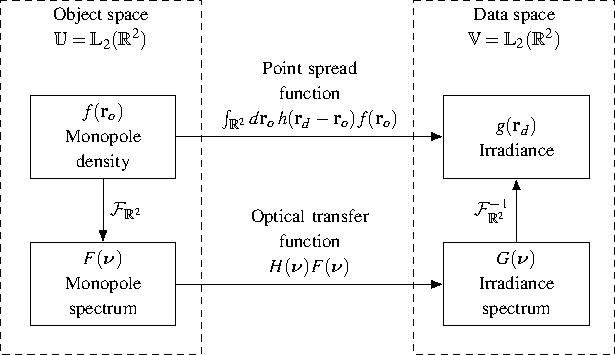
\includegraphics[scale=1.0]{../figures/monopole-block/monopole-block.pdf}
  \caption{
    The mapping between the object and data space of a monopole fluorescence microscope can be computed in two different bases---a delta function basis and a complex exponential basis. The change of basis can be computed with $n$-dimensional Fourier transforms denoted $\mathcal{F}_{\mbb{R}^n}$. Gray highlighting indicates which part of each expression is being named.
  }
  \label{fig:monopole-block}
\end{figure}

\subsubsection{Monopole coherent transfer functions}
The monopole point spread function can always be written as the absolute square of a monopole coherent spread function
\begin{align}
  |c(\rd - \roperp, \ropar)|^2 = h(\rd - \roperp, \ropar).
\end{align}
By applying the autocorrelation theorem we can use the monopole coherent transfer function as a shortcut for calculating the monopole transfer function
\begin{align}
  H(\bv) = \int_{\mbb{R}^3}d\bt\,C(\bt)C^*(\bt - \bv),
\end{align}
where $\bt = (\btperp, \btpar)$ is a three-dimensional transverse spatial frequency coordinate with its transverse/axial decomposition, and $C(\bt)$ is a coherent transfer function defined by
\begin{align}
  C(\bt) = \int_{\mbb{R}^3}d\bs{\mf{r}}\, c(\bs{\mf{r}})\,\text{exp}(-2\pi i\bs{\mf{r}}\cdot\bt).\label{eq:monoctf}
\end{align}
Figure \ref{fig:monopole-transfer-functions} summarizes the relationships between the transfer functions.  

\begin{figure}
  \centering
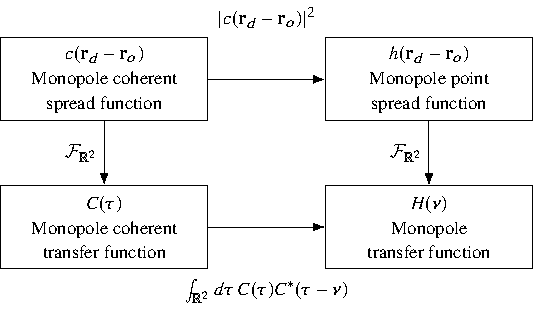
\includegraphics[scale=1.0]{../figures/monopole-transfer-functions/monopole-transfer-functions.pdf}
  \caption{
    The monopole transfer functions are related by a two-dimensional Fourier transform (right column). The coherent monopole transfer functions (left column) can be used to simplify the calculation of the remaining transfer functions.
  }
  \label{fig:monopole-transfer-functions}
\end{figure}

\subsubsection{Monopole pupil functions}
In this section we will relate the monopole transfer functions to physical
parameters. First, consider the field created at $\rs$ by a monopole at $\ro$
\begin{align}
  U_s(\rs, \ro) \propto \frac{\text{exp}[2\pi i\nu_m|\rs - \ro|]}{|\rs - \ro|},
\end{align}
where $\nu_m = n_o/\lambda$ is the radius of the Ewald sphere. For monopoles near the origin we can find the fields on the Gaussian reference sphere of an objectives lens with focal length $f_0 \gg |\ro|$ by applying the approximation $|\rs - \ro| \approx |\rs| - \rs\cdot\ro/|\rs|$ and dropping second-order amplitude and constant phase terms
\begin{align}
  U_s(\rs, \ro) \propto \frac{1}{f_0}\text{exp}[-2\pi i\nu_m(\rs\cdot\ro)/f_0].
\end{align}
Next, we expand the coordinates into transverse and axial components
\begin{align}
  U_s(\rs, \roperp, \ropar) \propto \frac{1}{f_0}\text{exp}[-2\pi i\nu_m(\rsperp\cdot\roperp + \rspar\ropar)/f_0],
\end{align}
then rewrite in pupil coordinates using the relationships $\rsperp = \rpperp$ and $\rspar = \sqrt{f_0^2 - |\rppar|^2}$
\begin{align}
  U_p(\rpperp, \roperp, \ropar) \propto \frac{1}{f_0}\text{exp}\left[-2\pi i\nu_m\left(\rpperp\cdot\roperp + \ropar\sqrt{f_0^2 - |\roperp|^2}\right)/f_0\right].
\end{align}
We can rewrite the field in the pupil plane as
\begin{align}
  U_p(\rpperp, \roperp, \ropar) \propto \frac{1}{f_0}p_d(\rpperp, \ropar)\,\text{exp}\left[-2\pi i \frac{n_0}{\lambda f_0}\rpperp\cdot\roperp\right],
\end{align}
where $p_d(\rpperp, \ropar)$ is the \textit{defocused monopole pupil function}  
\begin{align}
  p_d(\rpperp, \ropar) = p(\rpperp)\, \text{exp}\left[-2\pi i\nu_m\ropar\sqrt{1 - (|\rpperp|/f_0)^2}\right],
\end{align}
and $p(\rpperp)$ is the usual pupil function that can be used to model the angular cutoff, apodization, aberration, or phase masks.

Since the second lens is paraxial, we can model the relationship between the field in the pupil plane and the field on the detector with a scaled Fourier transform
\begin{align}
  U_d(\rdp, \roperp, \ropar) \propto \frac{n_1}{\lambda f_0f_1}\int_{\mbb{R}^2}d\rpperp\,p_d(\rpperp, \ropar)\,\text{exp}\left[-2\pi i \frac{n_0}{\lambda f_0}\rpperp\cdot\roperp\right]\text{exp}\left[-2\pi i \frac{n_1}{\lambda f_1}\rpperp\cdot\rdp\right].
\end{align}

If we define $P(\btperp, \ropar)$ as the two-dimensional transverse Fourier transform of the defocused pupil function
\begin{align}
  P(\btperp, \ropar) = \int_{\mbb{R}^2}d\rpperp\, p_d(\rpperp, \ropar)\,\text{exp}(-2\pi i \rpperp\cdot\btperp),\label{eq:pupilF}
\end{align}
then we can rewrite the field on the detector as
\begin{align}
  U_d(\rdp, \roperp, \ropar) \propto \frac{n_1}{\lambda f_0f_1}P\left(\frac{n_0}{\lambda f_0}\roperp + \frac{n_1}{\lambda f_1}\rdp, \ropar\right).
\end{align}
After rewriting in terms of the magnification $m = -\frac{f_1 n_0}{f_0 n_1}$, demagnifying the coordinates with $\rd = \rdp/m$, and demagnifying the irradiance with $h(\rd - \roperp, \ropar) \propto h'(m[\rd - \roperp], \ropar) $, we find the defocused monopole point spread function is related to the Fourier transform of the defocused monopole pupil function by 
\begin{align}
  h(\rd-\roperp, \ropar) \propto \left|\frac{n_1}{\lambda f_0f_1}P\left(-\frac{n_0}{\lambda f_0}[\rd - \roperp], \ropar\right)\right|^2.
\end{align}
The monopole point spread function is the absolute square of the monopole coherent spread function so
\begin{align}
  c(\rd - \roperp, \ropar) \propto \frac{n_1}{\lambda f_0f_1}P\left(-\frac{n_0}{\lambda f_0}[\rd - \roperp], \ropar\right). \label{eq:monocsf}
\end{align}
Our final task is to calculate the monopole coherent transfer function by plugging Eq. \eqref{eq:monocsf} into Eq. \eqref{eq:monoctf} which yields
\begin{align}
  C(\bt) \propto \frac{n_1}{\lambda f_0f_1}\int_{\mbb{R}}dr^{\mypar}\int_{\mbb{R}^2}d\mb{r}^{\bot}\, P\left(-\frac{n_0}{\lambda f_0}\mb{r}^{\bot}, r^{\mypar}\right)\,\text{exp}(-2\pi i[\mb{r}^{\bot}\cdot\btperp + r^{\mypar}\btpar]).
\end{align}
Using Eq. \eqref{eq:pupilF} to simplify the transverse integral yields
\begin{align}
  C(\bt) \propto \frac{1}{\nu_m}\, p\left(\frac{\lambda f_0}{n_0}\btperp\right) \int_{\mbb{R}}d r^{\mypar} \,\text{exp}\left(-2\pi i r^{\mypar}\sqrt{\nu_m - |\btperp|^2}\right)\,\text{exp}(-2\pi i r^{\mypar}\btpar).
\end{align}
Finally, we use the Fourier shift theorem to evaluate the axial integral to find that 
\begin{align}
  C(\bt) \propto \frac{1}{\nu_m}p\left(\frac{\lambda f_0}{n_0}\btperp\right)\,\delta\left(\btpar - \sqrt{\nu_m^2 - |\btperp|^2}\right).
\end{align}
This shows that the three-dimensional coherent transfer function is a scaled pupil function on a spherical cap. 


% \subsection{Three-dimensional dipole transfer functions}
% \subsubsection{Dipole transfer functions}
% \begin{figure}
%   \hspace{-6em}
%   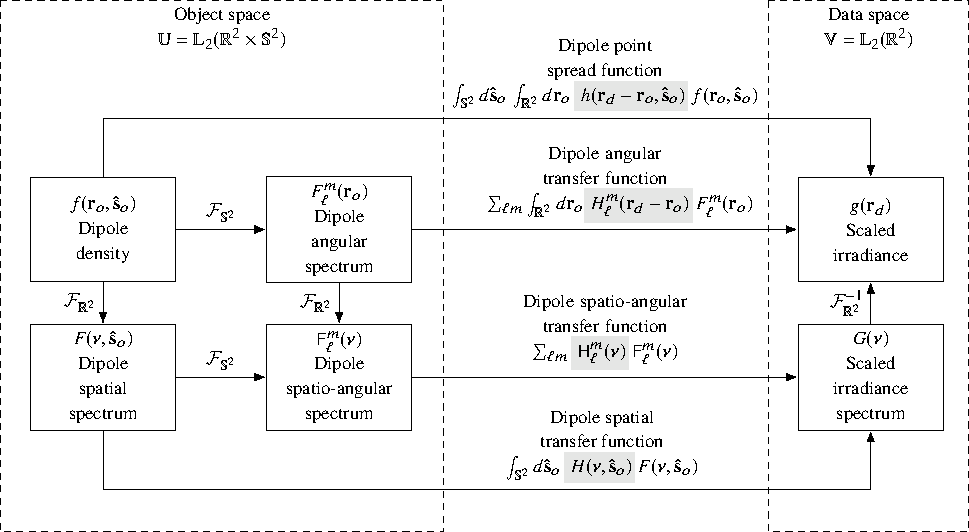
\includegraphics[scale=1.0]{../figures/dipole-block/dipole-block.pdf}
%   \caption{
%     % The mapping between the object space and data space of a dipole imaging system can be computed in four different bases---a delta function basis, a complex-exponential/angular-delta basis, a spatial-delta/spherical-harmonic basis, and a complex-exponential/spherical-harmonic basis. The changes of basis can be computed with the two-dimensional Fourier transform denoted $\mathcal{F}_{\mbb{R}^2}$, and the spherical Fourier transform denoted $\mathcal{F}_{\mbb{S}^2}$. Gray highlighting indicates which part of each expression is being named.
%   }
%   \label{fig:dipole-block}      
% \end{figure}

% \subsubsection{Dipole coherent transfer functions}

% \begin{figure}
%   \hspace{-2em}
% \includegraphics[scale=1.0]{../figures/dipole-transfer-functions/dipole-transfer-functions.pdf}
% \caption{
%   % There is one transfer function for each set of object-space basis functions, and these transfer functions are related by two-dimensional and spherical Fourier transforms---see center and right columns. There is an additional pair of coherent transfer functions that are useful for calculating the transfer functions---see left column.
% }
%   \label{fig:transfer-functions}
% \end{figure}

% \subsubsection{Dipole pupil functions}

\section{Results}
\subsection{Monopole transfer functions}
We can model an aplanatic microscope imaging monopole emitters with the scalar pupil function
\begin{align}
  p(\rpperp) \propto  \tilde{C}\left(\frac{|\rpperp|}{f_0}\right)\Pi\left(\frac{|\rpperp|}{2f_0\sin\alpha}\right), \label{eq:monopupil}
\end{align}
where
\begin{align}
  \tilde{C}(x) = (1 - x^2)^{-1/4}.
\end{align}
Plugging Eq. \eqref{eq:monopupil} in Eq. \eqref{eq:monoctf} yields
\begin{align}
  C(\bt) \propto \frac{1}{\nu_m}\tilde{C}\left(\frac{|\btperp|}{\nu_m}\right)\,\delta\left(\btpar - \sqrt{\nu_m^2 - |\btperp|^2}\right)\,\Pi\left(\frac{|\btperp|}{\nu_c}\right),\label{eq:toexpand}
\end{align}
where $\nu_c = 2\text{NA}/\lambda$ and $\text{NA} = n_0\sin\alpha$. Applying an identity from Appendix \ref{sec:delta} (Eq. \eqref{eq:sphereidentity}) allows us to write the coherent transfer function in spherical coordinates as 
\begin{align}
  C(\bt) \propto \frac{1}{\nu_m}\sqrt{\cos\theta_\tau}\,\delta\left(|\bt| - \nu_m\right)\,\Pi\left(\frac{\theta_\tau}{2\alpha}\right).
\end{align}

In Appendix \ref{sec:monoauto} we calculate the autocorrelation of the coherent transfer function and show that the monopole transfer function is given by
\begin{align}
  H(\bv) = 4\pi\sin^2(\alpha/2)\,\delta(|\bv|) + \frac{|\bvpar|}{\nu_m|\bv|}\sqrt{p^2 - 1}\,E\left(\beta_m, \frac{p}{\sqrt{p^2 - 1}}\right)\infty\left(\frac{|\bvperp|}{\nu_m}, \frac{|\bvpar|}{\nu_m}, \alpha\right),
\end{align}
where $E(\beta_m, k)  = \int_0^{\beta_m} d\phi\sqrt{1 - k^2\sin^2\phi}$ is an incomplete elliptic integral of the second kind and
\begin{align}
  p = \frac{2|\bvperp|}{\bvpar|\bv|}\sqrt{\nu_m^2 - (|\bv|/2)^2},\qquad
  \beta_m = \cos^{-1}\left(\frac{1}{p}\left[\frac{2\nu_m}{|\bvpar|}\cos\alpha + 1\right]\right),\nonumber\\ \infty(x, z, \alpha) = \Pi\left(\frac{|z|}{2(\sqrt{1 - (|x| - \sin\alpha)^2} - \cos\alpha)}\right).
\end{align}

We can also investigate the three-dimensional monopole transfer functions under the paraxial approximation by expanding the argument of the delta function in Eq. \eqref{eq:toexpand} about $|\btperp| = 0$ and dropping fourth- and higher-order terms \begin{align}
  C(\bt) \propp \frac{1}{\nu_m}\delta\left(\btpar - \nu_m + |\btperp|^2/2\nu_m\right)\,\Pi\left(\frac{|\btperp|}{\nu_c}\right).
\end{align}
In Appendix B we calculate the autocorrelation of the paraxial coherent transfer and show that the paraxial monopole transfer function is given by
\begin{align}
  H(\bv) \eqp \frac{\pi\nu_c^2}{4\nu_m^2}\delta(|\bv|) + \frac{4}{\nu_m}\text{nez}\left(\frac{|\bvperp|}{\nu_c}, \frac{2\nu_m|\bvpar|}{\nu_c^2}\right),
\end{align}
where
\begin{align}
 \text{nez}(x, z) = \frac{1}{2|x|}\text{Re}\left[\sqrt{1 - \left(\frac{|z|}{|x|} + |x|\right)^2}\right].
\end{align}

Figure 3 compares the high-aperture transfer function to the paraxial transfer function in their normalized forms. For extremely high numerical apertures $\alpha = \pi/2$ the high-aperture transfer function predicts an axial spatial frequency cutoff that is double the prediction of the paraxial model. Additionally, the high-aperture transfer function predicts a spatial frequency support that is a horn torus at $\alpha = \pi/2$ and a lemon-profiled torus for $\alpha < \pi/2$, while the paraxial transfer function predicts a scaled parabolic-lemon-profiled torus for all $\alpha$. 

\begin{figure}
  \centering
  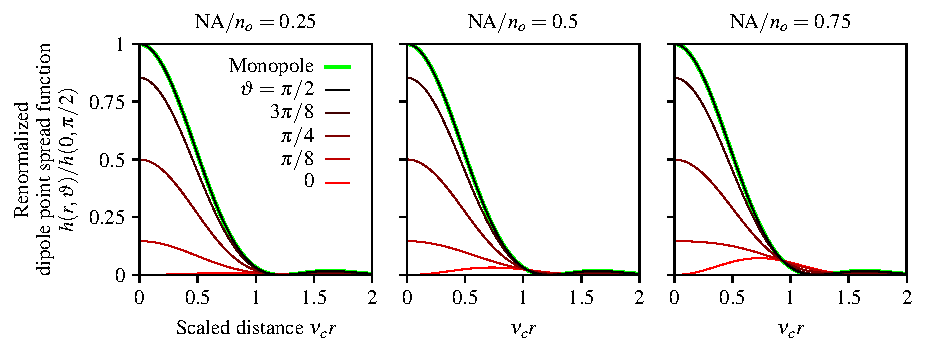
\includegraphics[scale=0.85]{../figures/monopole-psf/dpsf.pdf}
  \caption{Comparison of high-aperture and paraxial three-dimensional transfer functions for $\text{NA} = (1.00, 1.25, 1.50)$, $n_o = 1.5$, and $\lambda = 500\,\text{nm}$. Input spatial frequencies are in  m${}^{-1}$ and the output is in m${}^{+1}$. All transfer functions are normalized so that $\lim_{|{\bvperp}|\rightarrow 0} \int_\mbb{R}d\bvpar H(\bvperp, \bvpar) = 1$.}
  \label{fig:compare}
\end{figure}

% \subsection{Dipole transfer functions}
% \subsubsection{Dipole point spread function}

% \subsubsection{Dipole spatial transfer function}

% \subsubsection{Dipole angular transfer function}

% \subsubsection{Dipole spatio-angular transfer function}

\section{Discussion}
% Dipole phase masking:
% Azimuthal polarization filtering: \cite{lew2014}
% Metasurface polarization filtering: \cite{backlund2016}

\section{Conclusions}

\section*{Funding}
National Institute of Health (NIH) (R01GM114274, R01EB017293).

\section*{Acknowledgments}
TC was supported by a University of Chicago Biological Sciences Division Graduate Fellowship, and PL was supported by a Marine Biological Laboratory Whitman Center Fellowship. Support for this work was provided by the Intramural Research Programs of the National Institute of Biomedical Imaging and Bioengineering. 

\section*{Disclosures}
The authors declare that there are no conflicts of interest related to this article.

\bibliography{/Users/Talon/Library/texmf/talon}
\appendix

\section{Multidimensional curvilinear delta functions}\label{sec:delta}
In this appendix we summarize operational rules for manipulating multidimensional curvilinear delta functions. See Bracewell \cite{bracewell2004} for an intuitive approach to two-dimensional delta functions, and see Gelfand and Shilov \cite{gelfand2016} for a more mathematical discussion of multidimensional delta functions.

Our goal is to interpret delta functions of the form $\delta(\mb{g}(\mb{r}))$ where $\mb{g}: \mbb{R}^N \rightarrow \mbb{R}^M$. Starting with a simple case $N = M = 1$ and $g(r) = r$ we can use the sifting property to interpret the delta function
\begin{align}
  \int_{\mbb{R}}dr\,\delta(r)f(r) = f(0).
\end{align}
When $g(r) = ar$ then we can use a change of variables to show that 
\begin{align}
  \int_{\mbb{R}}dr\,\delta(ar)f(r) = \frac{f(0)}{|a|}.
\end{align}
Intuitively, the function $ar$ crosses its zero with an absolute slope $|a|$ so it sifts less of the function $f(r)$ by a factor of $|a|^{-1}$. 

When $g(r)$ is a function with multiple zeros then the delta functions sifts (with appropriate weighting) at all of the function's zeros 
\begin{align}
  \int_{\mbb{R}}dr\,\delta(g(r))f(r) = \sum_{g(r_i) = 0}f(r_i)\left|\frac{dg(r_i)}{dr}\right|^{-1}.\label{eq:zero1}
\end{align}

When $N > 1$ and $M = 1$ we can interpret the delta function as sifting over the (potentially infinite) set of zeros of $g(\mb{r})$
\begin{align}
  \int_{\mbb{R}^N}d\mb{r}\,\delta(g(\mb{r}))f(\mb{r}) = \int_{g^{-1}(0)}d\sigma(\mb{r})f(\mb{r})|\nabla g(\mb{r})|^{-1},\label{eq:zero2}
\end{align}
where $d\sigma(\mb{r})$ is an appropriate measure for the solution set, and $|\nabla g(\mb{r})|$ denotes the gradient magnitude evaluated at $\mb{r}$.

When $M > 1$ then $\mb{g}$ is a vector-valued function, and $\delta(\mb{g}(\mb{r})$ can be used to manipulate the product of multiple delta functions. For example, we can rewrite $\delta(g_1(\mb{r}))\delta(g_2(\mb{r}))$ as $\delta(\mb{g}(\mb{r}))$. When $N = M > 1$ 
we interpret the delta function in a familiar way
\begin{align}
  \int_{\mbb{R}^N}d\mb{r}\,\delta(\mb{g}(\mb{r}))f(\mb{r}) = \int_{\mb{g}^{-1}(0)}d\sigma(\mb{r})f(\mb{r})\left|\frac{\partial(g_1,\dots,g_M)}{\partial(r_1,\dots,r_N)}(\mb{r})\right|^{-1},
\end{align}
where $\left|\frac{\partial(g_1,\dots,g_M)}{\partial(r_1,\dots,r_N)}(\mb{r})\right|$ denotes the Jacobian determinant evaluated at $\mb{r}$.

The final case we will consider is when $N > M > 1$ which we can interpret with
\begin{align}
  \int_{\mbb{R}^N}d\mb{r}\,\delta(\mb{g}(\mb{r}))f(\mb{r}) = \int_{\mb{g}^{-1}(0)}d\sigma(\mb{r})f(\mb{r})\left|\frac{\partial(g_1,\dots,g_M)}{\partial(r^*_1,\dots,r^*_M)}(\mb{r})\right|^{-1},\label{eq:transversedelta}
\end{align}
where $r_1^*,\dots,r_M^*$ form an orthogonal basis for the tangent space of the solution set $\mb{g}^{-1}(0)$, and $\left|\frac{\partial(g_1,\dots,g_M)}{\partial(r^*_1,\dots,r^*_M)}(\mb{r})\right|$ denotes the Jacobian determinant in the tangent space evaluated at $\mb{r}$. For example, if $N = 3$, $M = 2$ and $\mb{g}(\mb{r}) = [2x, 3z]$, then the solution set is the $y$ axis. We can use the $x$ and $z$ unit vectors as a basis for the tangent space of the solution set, so we can write
\begin{align}
  \int_{\mbb{R}^3}dxdydz\,\delta\left(\begin{bmatrix}2x\\3z\end{bmatrix}\right)f(x,y,z) = \frac{1}{6}\int_{\mbb{R}}dy f(0,y,0).
\end{align}

In these examples we have been interpreting delta functions by sifting functions with a one-dimensional output $f:\mbb{R}^N\rightarrow \mbb{R}$, but these interpretations work equally well for functions with multidimensional outputs $\mb{f}:\mbb{R}^N\rightarrow \mbb{R}^P$.

The rules in this section can be used to manipulate delta functions that appear outside integrals. For example, we can use Eq. \eqref{eq:zero1} to verify the identity
\begin{align}
  \delta(x^2 - 1) = \frac{1}{2}[\delta(x - 1) + \delta(x + 1)]. 
\end{align}
Similar identities can be established for any multidimensional delta function by taking care that both the solution set and the appropriate Jacobian determinant are preserved. For example, we can use Eq. \eqref{eq:zero2} to verify that
\begin{align}
   \delta\left(\btpar \pm \sqrt{\nu_m^2 - |\btperp|^2}\right) = \frac{\btpar}{\nu_m}\delta\left(|\bt| - \nu_m\right) = \cos\theta_\tau\delta\left(|\bt| - \nu_m\right).\label{eq:sphereidentity}
\end{align}


\section{Coordinate systems for evaluating the autocorrelation of a spherical cap}\label{sec:coord}
In this appendix specify three coordinate systems which will be useful for evaluating the autocorrelation of spherical caps. By inspection of Fig. \ref{fig:caps}, the intersection of the two shifted spherical caps is a circular arc centered on the origin in the plane perpendicular to the shift direction $\bv$. To integrate along this arc it will be convenient to define two spherical coordinate systems defined with respect to the centers of the shifted spheres and a cylindrical coordinate system with its long axis parallel to the shift direction $\bv$. The shifted spherical coordinate systems are straightforward to derive as
\begin{align}
  \begin{bmatrix}
    \tau_x\\
    \tau_y\\
    \btpar
  \end{bmatrix}
  =
  \begin{bmatrix}
    |\bt|_{1,2}\sin\theta_{\tau_{1,2}}\cos\phi_{\tau_{1,2}} \pm \nu_x/2\\
    |\bt|_{1,2}\sin\theta_{\tau_{1,2}}\sin\phi_{\tau_{1,2}} \pm \nu_y/2\\
    |\bt|_{1,2}\cos\theta_{\tau_{1,2}} \pm \bvpar/2
  \end{bmatrix},\label{eq:spherical}
\end{align}
where the subscripts and $\pm$ indicate which of the pair of shifted coordinate systems we are using.

Deriving the cylindrical coordinate system is more involved. We follow Arnison and Sheppard \cite{arnison2002} and define a cylindrical coordinate system for shifts along the $x$ axis $\bv = (1,0,0)$ then generalize to arbitrary shifts by multiplying with rotation matrices
\begin{align}
  \begin{bmatrix}
    \tau_x\\
    \tau_y\\
    \btpar
  \end{bmatrix}
&= \mb{R}_{\mb{z}}(-\tan^{-1}(\nu_y/\nu_x)\mb{R}_{\mb{y}}(\sin^{-1}(\bvpar/|\bv|))\begin{bmatrix}
    \tau_\xi\\
    \tau_R\sin\beta_\tau\\
    -\tau_R\cos\beta_\tau
  \end{bmatrix},
\end{align}
where
\begin{align}
  \mb{R}_\mb{z}(\theta) =
  \begin{bmatrix}
    \cos\theta & 0 & -\sin\theta\\
    0 & 1 & 0\\
    \sin\theta & 0 &\cos\theta
  \end{bmatrix}\, ,\quad 
  \mb{R}_\mb{y}(\theta) =
  \begin{bmatrix}
    \cos\theta & \sin\theta & 0\\
    -\sin\theta & \cos\theta & 0\\
    0 & 0 & 1
  \end{bmatrix}  .
\end{align}
Multiplying the matrices and simplifying yields
\begin{align}
    \begin{bmatrix}
    \tau_x\\
    \tau_y\\
    \btpar
  \end{bmatrix}
  &=
  \begin{bmatrix}
    \displaystyle\frac{\nu_x}{|\bv|}\tau_\xi + \frac{\tau_R}{|\bvperp||\bv|}(\bvpar\nu_x\cos\beta_\tau - |\bv|\nu_y\sin\beta_\tau)\\[1em]
    \displaystyle\frac{\nu_y}{|\bv|}\tau_\xi + \frac{\tau_R}{|\bvperp||\bv|}(\bvpar\nu_y\cos\beta_\tau + |\bv|\nu_x\sin\beta_\tau)\\[1em]
    \displaystyle\frac{\bvpar}{|\bv|}\tau_\xi - \frac{|\bvperp|\tau_R}{|\bv|}\cos\beta_\tau
  \end{bmatrix}.\label{eq:cylindrical}
\end{align}

\begin{figure}
  \centering
  \includegraphics[scale=0.3]{../figures/caps/general.pdf}
  \includegraphics[scale=0.25]{../figures/caps/spherical.pdf}\hspace{0.5em}
  \includegraphics[scale=0.28]{../figures/caps/cylindrical.pdf}
  \caption{Geometric constructions and coordinate systems for performing the three-dimensional autocorrelation. (Top) Two spherical caps with spherical radius $\nu_m = n_o/\lambda$ and base diameter $\nu_c = 2\text{NA}/\lambda$ are shifted by $\bv$ and intersect along a circular arc in the plane perpendicular to $\bv$. (Bottom left) We define a spherical coordinate system for each cap. These coordinate systems  are most convenient for expressing the individual coherent transfer functions. (Bottom right) We define a cylindrical coordinate system with the long axis of the cylinder parallel to the shift direction $\bv$ and the azimuthal angle $\beta_\tau$ defined with respect to the lowest point of each cylindrical slice. This coordinate system is most convenient for integrating over the circular arc of intersection.}
  \label{fig:caps}
\end{figure}

\section{Three-dimensional monopole transfer functions}\label{sec:monoauto}
In this appendix we calculate the three-dimensional monopole transfer function
by evaluating the integral
\begin{align}
  H(\bv) \propto \int_{\mbb{R}^3}d\bt\, C(\bt + \bv/2)\,C^*(\bt - \bv/2). \label{eq:3dauto}
\end{align}
where the coherent transfer function is
\begin{align}
  C(\bt) \propto \,\frac{1}{\nu_m}\sqrt{\cos\theta_{\tau}}\,\delta\left(|\bt| - \nu_m\right)\,\Pi\left(\frac{\theta_{\tau}}{2\alpha}\right).\label{eq:3dctf2}
\end{align}
We can interpret the integral in Eq. \eqref{eq:3dauto} as the autocorrelation of a $\sqrt{\cos\theta_\tau}$-weighted spherical cap with radius $\nu_m$ and half angle $\alpha$.

First, we plug Eq. \eqref{eq:3dctf2} into Eq. \eqref{eq:3dauto}, rewrite the delta functions in vector notation, and use the shifted spherical coordinates from Appendix \ref{sec:coord}
\begin{align}
  H(\bv) \propto \frac{1}{\nu_m^2}\int_{\mbb{R}^3}d\bt\,\delta\left(\begin{bmatrix}|\bt + \bv/2| - \nu_m\\ |\bt - \bv/2| - \nu_m \end{bmatrix}\right)\sqrt{\cos\theta_{\tau_1}\cos\theta_{\tau_2}}\,\Pi\left(\frac{\theta_{\tau_1}}{2\alpha}\right)\Pi\left(\frac{\theta_{\tau_2}}{2\alpha}\right).
\end{align}
Next, we calculate all of the pieces we need to apply Eq. \eqref{eq:transversedelta} from Appendix \ref{sec:delta}. First, the argument of the delta function is zero on a circle with radius $\nu_\circ = \sqrt{\nu_m^2 - (|\bv|/2)}$. We will integrate over the circle in cylindrical coordinates (see Appendix \ref{sec:coord}) using the measure $\nu_\circ d\beta_\tau$. Next, we calculate the transverse Jacobian determinant on the circle of intersection. The transverse Jacobian determinant will be the same for all points around the circle of intersection and for all shift directions (by the symmetry of the spheres), so we only calculate the transverse Jacobian for shifts along the $\mb{x}$ axis at the point of intersection $\bs{\tau}^* = [0, 0, \nu_\circ]$. We will use the $x$ and $z$ directions as a basis for the tangent space and calculate the transverse Jacobean determinant as
\begin{align}
  \left|\begin{bmatrix}\frac{\partial g_1}{\partial x}(\bs{\tau}^*)&\frac{\partial g_1}{\partial z}(\bs{\tau}^*)\\\frac{\partial g_2}{\partial x}(\bs{\tau}^*)&\frac{\partial g_2}{\partial z}(\bs{\tau}^*)\end{bmatrix}\right| = \left|\begin{bmatrix}\frac{-|\bv|}{2\nu_m}&\frac{\nu_\circ}{\nu_m}\\\frac{|\bv|}{2\nu_m}&\frac{\nu_\circ}{\nu_m}\end{bmatrix}\right| = \frac{|\bv|\nu_\circ}{\nu_m^2}.
\end{align}
Bringing the solution set, the measure, and the inverse transverse Jacobian together yields
\begin{align}
  H(\bv) = \frac{1}{|\bv|}\int_0^{2\pi} d\beta_\tau\,\sqrt{\cos\theta_{\tau_1}\cos\theta_{\tau_2}}\,\Pi\left(\frac{\theta_{\tau_1}}{2\alpha}\right)\Pi\left(\frac{\theta_{\tau_2}}{2\alpha}\right).\label{eq:lastform}
\end{align}

Next, we express the integrand in terms of $\beta_\tau$. Equating the $\btpar$ components in Eqs. \eqref{eq:spherical} and \eqref{eq:cylindrical} and evaluating on the circle of intersection ($|\bt|\rightarrow \nu_m$, $\tau_\xi\rightarrow 0$, $\tau_R\rightarrow \nu_\circ$) yields the relationship
\begin{align}
  \nu_m\cos\theta_{\tau_{1,2}} \pm \frac{\bvpar}{2} = -\frac{|\bvperp|\nu_\circ}{|\bv|}\cos\beta_\tau\label{eq:angles}.
\end{align}
The integrand is written in terms of $\cos\tau_{\theta_{1,2}}$, so we rewrite Eq. \eqref{eq:angles} to find the relationship
\begin{align}
  \cos\theta_{\tau_{1,2}} = \frac{1}{\nu_m}\left(-\frac{|\bvperp|\nu_\circ}{|\bv|}\cos\beta_\tau\mp \frac{\bvpar}{2}\right) = \frac{\bvpar}{2\nu_m}\left(-p\cos\beta_\tau \mp 1\right)
\end{align}
where
\begin{align}
  p = \frac{2|\bvperp|\nu_\circ}{\bvpar|\bv|}.
\end{align}

We can also use Eq. \eqref{eq:angles} to find the limits of integration for $\beta_\tau$ by setting $\tau_{\theta_2} \rightarrow \alpha$ then solving for $\beta_\tau$ to find the maximum azimuthal angle $\beta_m$
\begin{align}
  \beta_m = \cos^{-1}\left[\frac{1}{p}\left(\frac{2\nu_m}{|\bvpar|}\cos\alpha + 1\right)\right].
\end{align}

Now that we have written the integrand in terms of $\beta_tau$, we can write Eq. \eqref{eq:lastform} as
\begin{align}
  H(\bv) \propto \frac{\bvpar}{|\bv|\nu_m}\int_{0}^{\beta_m}d\beta_\tau\, \sqrt{p^2\cos^2\beta_\tau - 1}, 
\end{align}
which can be written as 
\begin{align}
  H(\bv) \propto \frac{\bvpar}{|\bv|\nu_m}\sqrt{p^2 - 1}\,E\left(\beta_m, \frac{p}{\sqrt{p^2 - 1}}\right), \label{eq:intresult}
\end{align}
where $E(\beta_m, k)  = \int_0^{\beta_m} d\phi\sqrt{1 - k^2\sin^2\phi}$ is an incomplete elliptic integral of the second kind.

The spherical shells only intersect when 
\begin{align}
|\bvpar| < \sqrt{\nu_m^2 - (|\bvperp| - \nu_m\sin\alpha)^2} - \nu_m\cos\alpha, 
\end{align}
so the transfer function will be zero when this condition is not satisfied.
We can rewrite this condition conveniently by defining a function
\begin{align}
  \infty(x, z, \alpha) = \Pi\left(\frac{|z|}{2(\sqrt{1 - (|x| - \sin\alpha)^2} - \cos\alpha)}\right).
\end{align}

The result in Eq. \eqref{eq:intresult} diverges as $|\bv| \rightarrow 0$ so the transfer function is still undefined at that point. Instead, we calculate the value of the transfer function at $\bv = 0$ by applying the central-ordinate theorem. The solid angle of the sphere collected by the optical system is the value of the transfer functions $\bv = 0$ so $H(0) = 4\pi\sin^2(\alpha/2)$.

Stitching together the two solutions and accounting for the region of validity yields the complete transfer function
\begin{align}
  H(\bv) \propto 4\pi\sin^2(\alpha/2)\,\delta(|\bv|) + \frac{|\bvpar|}{\nu_m|\bv|}\sqrt{p^2 - 1}\,E\left(\beta_m, \frac{p}{\sqrt{p^2 - 1}}\right)\infty\left(\frac{|\bvperp|}{\nu_m}, \frac{\bvpar}{\nu_m}, \alpha \right).
\end{align}

Next, we calculate the monopole transfer function under the paraxial approximation. We approximate the $\sqrt{\cos\theta_\tau}$-weighted spherical cap with a truncated paraboloid
\begin{align}
  C(\bt) \propp \frac{1}{\nu_m}\delta\left(\btpar - \nu_m + |\btperp|^2/2\nu_m\right)\,\Pi\left(\frac{|\btperp|}{\nu_c}\right). \label{eq:ctf}
\end{align}

For the high-aperture case we evaluated the three-dimensional autocorrelation
directly, but for the paraxial case it is easier to evaluate the two-dimensional
autocorrelation of the defocused coherent transfer functions. We rewrite the
three-dimensional transfer function as
\begin{align}
  H(\bv) = \int_{\mbb{R}}dr^{\mypar}\,H^{(d)}(\bvperp,r^{\mypar})\,\text{exp}(-2\pi i r^{\mypar}\bvpar),\label{eq:def3dtf}
\end{align}
where $H^{(d)}(\bvperp,r^{\mypar})$ is the defocused transfer function given by
\begin{align}
  H^{(d)}(\bvperp,r^{\mypar}) = \int_{\mbb{R}^2}d\btperp\,C^{(d)}(\btperp + \bvperp/2, r^{\mypar})C^{(d)*}(\btperp - \bvperp/2, r^{\mypar}), \label{eq:defautocorr}
\end{align}
and $C^{(d)}(\btperp, r^{\mypar})$ is the defocused coherent transfer function given by
\begin{align}
  C^{(d)}(\btperp, r^{\mypar}) = \int_{\mbb{R}}d\btpar\, C(\bt)\,\text{exp}(2\pi i r^{\mypar}\btpar).\label{eq:deftf}
\end{align}
We plug Eq. \eqref{eq:ctf} into Eq. \eqref{eq:deftf} and evaluate the Fourier transform to find that the defocused coherent transfer function is
\begin{align}
  C^{(d)}(\btperp, r^{\mypar}) \propp \frac{1}{\nu_m}\text{exp}(2\pi i r^{\mypar}[-\nu_m + |\btperp|^2/2\nu_m])\Pi\left(\frac{|\btperp|}{\nu_c}\right), \label{eq:defctf}
\end{align}
which we can interpret as a disk with uniform magnitude and a quadratic phase factor that depends on the defocus $r^{\mypar}$. 

Next, we evaluate the defocused transfer function by plugging Eq. \eqref{eq:defctf} into Eq. \eqref{eq:defautocorr} and simplifying the complex exponentials
\begin{align}
  H^{(d)}(\bvperp,r^{\mypar}) \propp \frac{1}{\nu_m^2}\int_{\mbb{R}^2}d\btperp\, \text{exp}(2\pi i r^{\mypar}[\btperp\cdot\bvperp/\nu_m])\Pi\left(\frac{|\btperp + \bvperp/2|}{\nu_c}\right) \Pi\left(\frac{|\btperp - \bvperp/2|}{\nu_c}\right).\label{eq:defocusresult}
\end{align}
Plugging Eq. \eqref{eq:defocusresult} into Eq. \eqref{eq:def3dtf} and evaluating the
Fourier transform yields 
\begin{align}
  H(\bv) \propp \frac{1}{\nu_m^2}\int_{\mbb{R}^2}d\btperp\, \delta(\bvpar - \btperp\cdot\bvperp/\nu_m)\Pi\left(\frac{|\btperp + \bvperp/2|}{\nu_c}\right) \Pi\left(\frac{|\btperp - \bvperp/2|}{\nu_c}\right).
\end{align}
\begin{figure}
  \centering
  \includegraphics[scale=0.2]{../figures/para-geometry/para-geometry.pdf}
  \caption{Geometric construction for evaluating the three-dimensional autocorrelation under the paraxial approximation. We need to integrate over a line perpendicular to the transverse shift direction $\bvperp$ that is displaced from the origin by $\nu_m|\bvpar|/|\bvperp|$ and truncated by the shifted circles with diameter $\nu_c$.}
  \label{fig:geometry}
\end{figure}

We can evaluate this integral with the help of the geometric construction in Fig. \ref{fig:geometry}. The delta function corresponds to a line perpendicular to the transverse shift direction $\bvperp$ displaced from the origin by $\nu_m|\bvpar|/|\bvperp|$. Within the intersection of the shifted circles this line has length $2\sqrt{(\nu_c/2)^2 - ([\nu_m|\bvpar|/|\bvperp|] + [|\bvperp|/2])^2}$. Finally, the transverse Jacobian (the transverse derivative in this case) of the function is $|\bvperp|/\nu_m$, so the integral evaluates to 
\begin{align}
  H(\bv) \propp \frac{2}{\nu_m|\bvperp|}\sqrt{\left(\frac{\nu_c}{2}\right)^2 - \left(\frac{\nu_m|\bvpar|}{|\bvperp|} + \frac{|\bvperp|}{2}\right)^2}. \label{eq:intresult3}
\end{align}

The truncated paraboloids only intersect when
\begin{align}
  |\bvpar| < -\frac{1}{2\nu_m}|\bvperp|(|\bvperp| - \nu_c),
\end{align}
so the paraxial transfer function is zero when this condition is not satisfied. We can incorporate this condition conveniently by only considering the real part of the expression in Eq. \eqref{eq:intresult3}.

Once again, the result in Eq. \eqref{eq:intresult3} diverges as $|\bv| \rightarrow 0$, but we can use the central-ordinate theorem to find that $H(0) = \frac{\pi\nu_c^2}{4\nu_m^2}$. 

The complete paraxial transfer function is 
\begin{align}
  H(\bv) \propp \frac{\pi\nu_c^2}{4\nu_m^2}\delta(|\bv|) + \frac{2}{\nu_m|\bvperp|}\text{Re}\left\{\sqrt{\left(\frac{\nu_c}{2}\right)^2 - \left(\frac{\nu_m|\bvpar|}{|\bvperp|} + \frac{|\bvperp|}{2}\right)^2}\right\}.
\end{align}
We can rewrite the paraxial transfer function in a scaled form 
\begin{align}
  H(\bv) \eqp \frac{\pi\nu_c^2}{4\nu_m^2}\delta(|\bv|) + \frac{4}{\nu_m}\text{nez}\left(\frac{|\bvperp|}{\nu_c}, \frac{2\nu_m|\bvpar|}{\nu_c^2}\right),
\end{align}
where we have defined the function
\begin{align}
 \text{nez}(x, z) = \frac{1}{2|x|}\text{Re}\left[\sqrt{1 - \left(\frac{|z|}{|x|} + |x|\right)^2}\right]
\end{align}
and named it for its resemblance to pince-nez (nose-pinching glasses)---see Fig. \ref{fig:nez}.
\begin{figure}
  \centering
  \includegraphics[scale=0.9]{../figures/nez/nez.pdf}
  \caption{Plot of $\text{nez}(x,z)$ with contours on integer values between 0 and 5. $\text{nez}(x,z)$ has a singularity at the origin, so we have truncated values above 10.}
  \label{fig:nez}
\end{figure}

We can recover the two-dimensional paraxial transfer function by integrating over the axial coordinate
\begin{align}
  H(\bvperp) \eqp \int_{\mbb{R}}d\bvpar\, H(\bv) = \frac{4\nu_c^2}{\pi\nu_m^2}\text{chat}_0\left(\frac{|\bvperp|}{\nu_c}\right), 
\end{align}
where we have used
\begin{align}
  \int_{\mbb{R}}dz\,\text{nez}(x,z) = \text{chat}_0(x) = \frac{1}{2}\left[\cos^{-1}|x| - |x|\sqrt{1-x^2}\right]\Pi\left(\frac{x}{2}\right).
\end{align}
\end{document}
